\begin{center}
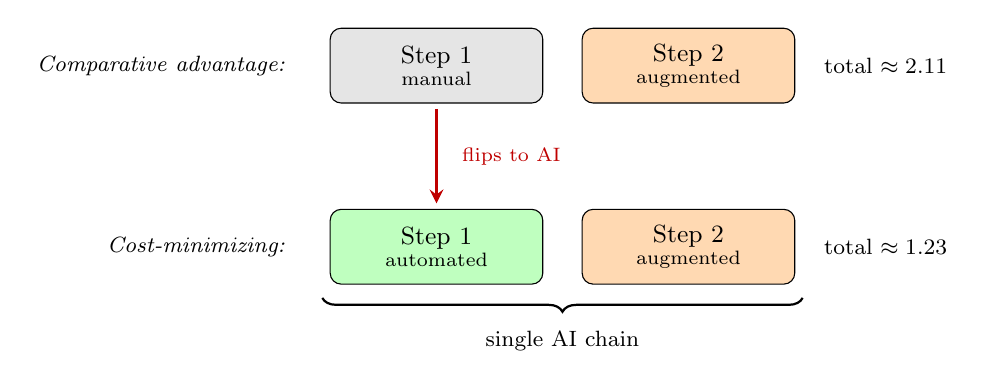
\begin{tikzpicture}[>=stealth,
  cbox/.style={rectangle, rounded corners, draw, minimum width=2.7cm, minimum height=0.95cm, align=center, font=\small}]
  % row labels
  \node[font=\footnotesize\itshape, anchor=east] at (1.4, 0)    {Comparative advantage:};
  \node[font=\footnotesize\itshape, anchor=east] at (1.4, -2.3) {Cost-minimizing:};
  % row 1: assign each step to its cheaper factor in isolation
  \node[cbox, fill=gray!20]   (a1) at (3.2, 0) {Step 1\\[-3pt]{\scriptsize manual}};
  \node[cbox, fill=orange!30] (a2) at (6.4, 0) {Step 2\\[-3pt]{\scriptsize augmented}};
  \node[font=\footnotesize, anchor=west] at (8.0, 0) {total $\approx 2.11$};
  % row 2: optimal -- both chained, step 1 automated
  \node[cbox, fill=green!25]  (b1) at (3.2, -2.3) {Step 1\\[-3pt]{\scriptsize automated}};
  \node[cbox, fill=orange!30] (b2) at (6.4, -2.3) {Step 2\\[-3pt]{\scriptsize augmented}};
  \draw[thick, decorate, decoration={brace, amplitude=5pt, mirror}] (1.75, -2.95) -- (7.85, -2.95);
  \node[font=\footnotesize] at (4.8, -3.5) {single AI chain};
  \node[font=\footnotesize, anchor=west] at (8.0, -2.3) {total $\approx 1.23$};
  % step 1 flips from manual to automated
  \draw[->, very thick, red!75!black] (3.2, -0.55) -- (3.2, -1.75);
  \node[font=\scriptsize, text=red!75!black, anchor=west] at (3.4, -1.15) {flips to AI};
\end{tikzpicture}
\end{center}
